\begin{center}
    \section*{\fontsize{20}{20}\selectfont Chapter 3}
\end{center}
\vspace{10mm}
\section{Research Methodology}

This chapter represents the methodology adopted for this research to identify the behavioral patterns of children related or heavily suspected to autism disorder. The approach taken for this purpose is a structured pipeline from collecting the video data to making the model prediction and evaluation in the end. The computer vision approach is taken for extracting the pose-based features from the video data and then the classification of certain poses is done using the machine learning and deep learning models.

\subsection{Proposed Framework}

The proposed framework consists of some interconnected modules that process raw video data and transform it then results into meaningful behavioral predictions. The framework starts with short video clips that contain autism-related behaviors. The video data is then fed into the pose estimation module to obtain human body landmarks. These landmarks are then used to create fixed length temporal sequences.

Two parallel modeling methods have been used. For the first method, statistical features are extracted from the pose sequence data and classical machine learning models are then trained. For the second method, sequence-based deep learning models are trained directly on the pose sequence data to learn about temporal dependencies. Finally, the system has used multiple metrics to evaluate the models performance and provides the probabilities for each class in the predictions.

Figure~\ref{fig:detail_workflow} illustrates the overall workflow of the proposed framework.

\begin{figure}[htbp]
\centering
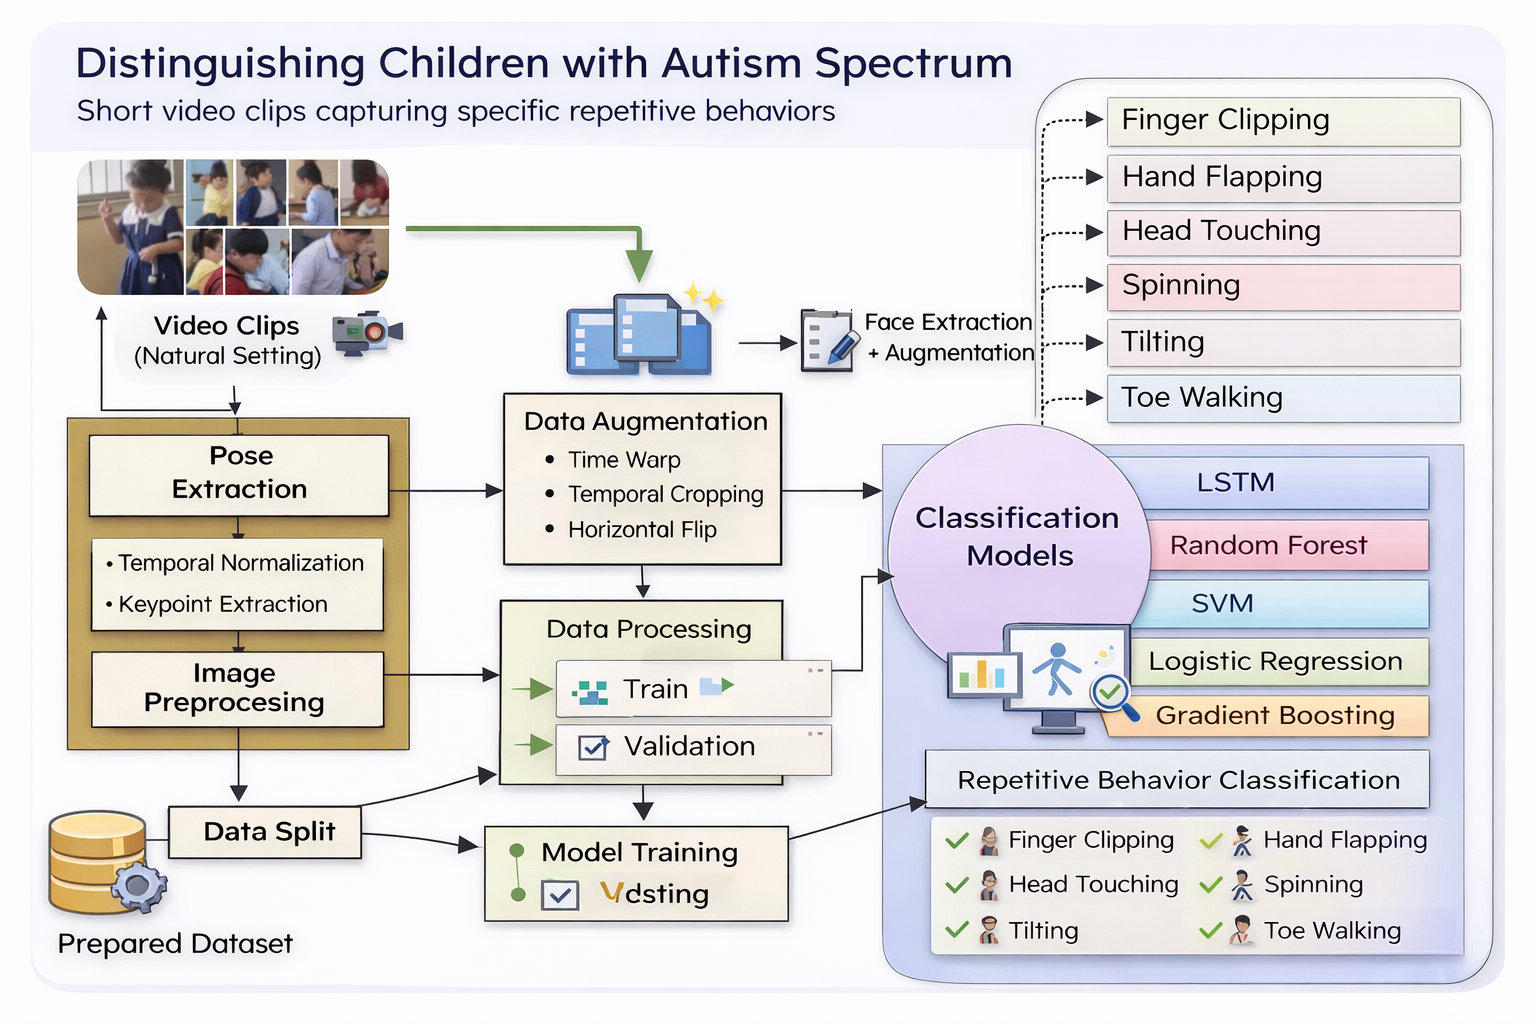
\includegraphics[scale=0.25]{image/example_arch.png}
\caption{Workflow of the Proposed Autism Behavior Detection Framework}
\label{fig:detail_workflow}
\end{figure}

\subsection{Data Set Analysis}

The dataset which is used for this research consists of private videos of certain behaviour poses of children with autism-related behavioral patterns. The videos are short in duration, typically ranging between 1 to 4 seconds. The videos are short and concentrate for specific behavioral actions.Thus it erffectivly reduces the background noise and emphasizes on the motion patterns.Beside, when the subjects display these certain behaviors, the video recording had to be with the exact timing.

All these videos are processed to extract the pose landmarks by using the MediaPipe Pose library. There are 33 body landmarks in every frame, where every landmark is defined by the x-coordinate, y-coordinate and the visibility score. To ensure consistency, all the videos are converted into fixed length sequences of 30 frames.

\begin{table}[htbp]
\caption{Autism-Related Behavioral Classes in the Dataset}
\begin{center}
\begin{tabularx}{0.6\textwidth}{
| >{\centering\arraybackslash}X
| >{\centering\arraybackslash}X | }
\hline
\textbf{Class Label} & \textbf{Behavior Description} \\
\hline
finger\_cliping & Repetitive finger movement behavior \\
\hline
hand\_flapping & Rapid hand movement behavior \\
\hline
head\_touching & Repetitive touching of head \\
\hline
spining & Rotational body movement \\
\hline
tilting & Repeated body or head tilting \\
\hline
head\_touching & Repeated head or face touching via hand \\
\hline
\end{tabularx}
\label{tab:dataset_classes}
\end{center}
\end{table}

\subsubsection{Data Collection and Preprocessing}

The video data was collected using Samsung A1 Android Mobile
devices camera from a disabled children school located at Mirpur coordinates in 23.933799633727386, 90.24442128295833 with appropriate with the consent of the school authority and the respected gurdian of the children and also by taking the consent from the respective parents and school authorities. Videos are resized and converted to RGB format before the extraction of the poses. MediaPipe Pose is used here for the project for the detection of body landmarks from the videos.

Over 50 childen has been crucial for this thesis and their data has been very important. 

\begin{figure}[htbp]
\centering
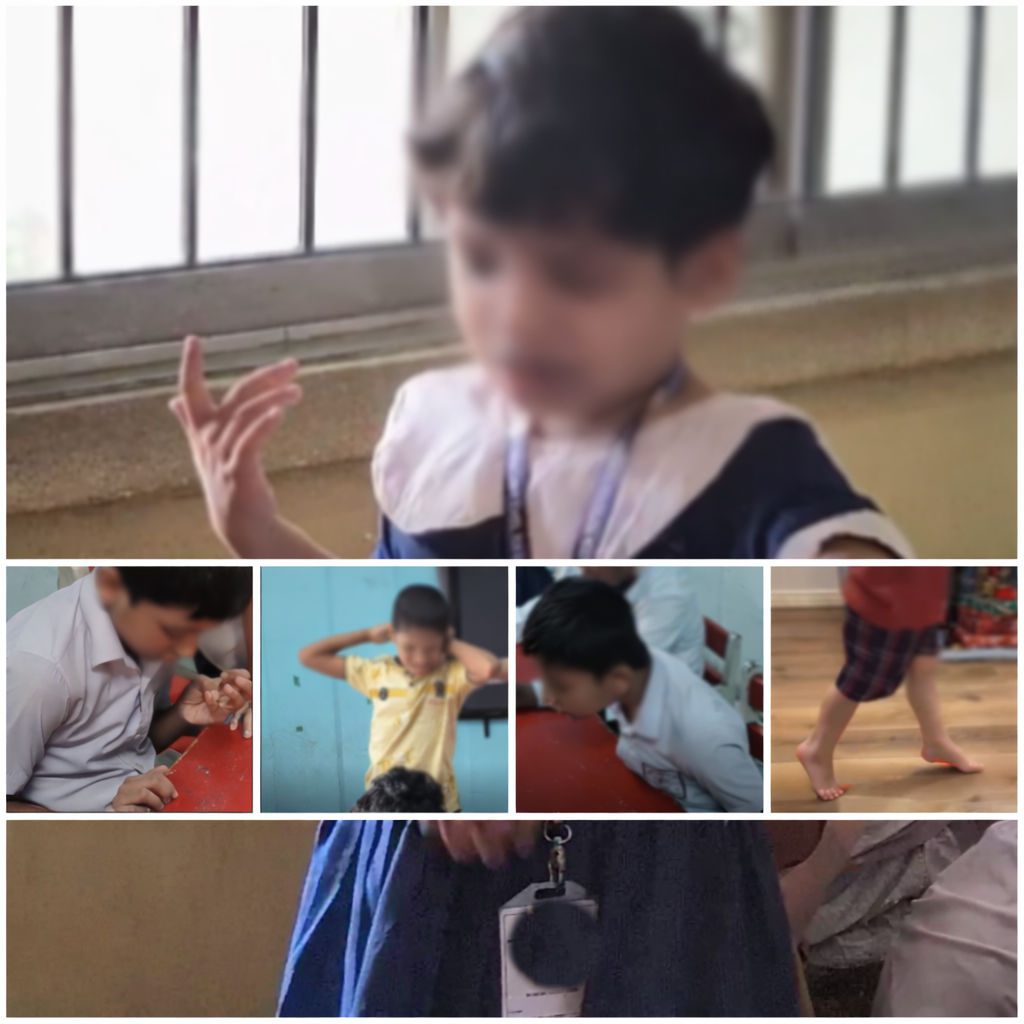
\includegraphics[scale=0.25]{image/college.png}
\caption{Sample Datset Image Demonstrating Poses}
\label{fig:sample_images_of_the_children}
\end{figure}

As shown in Figure~\ref{fig:sample_images_of_the_children} the back image of the four, the child is caught doing handflapping and finger cliping both and also in these four images children are doing finger cliping, head touching, tilting and also toe walking which are very much self explanatory.

\begin{figure*}[htbp]
\centering

\begin{subfigure}{0.32\textwidth}
    \centering
    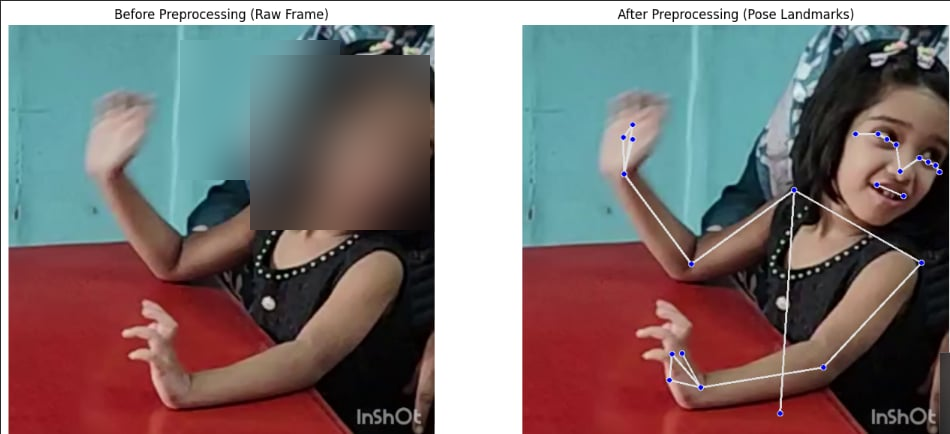
\includegraphics[width=\linewidth]{image/preprocess1.png}
\end{subfigure}
\hfill
\begin{subfigure}{0.32\textwidth}
    \centering
    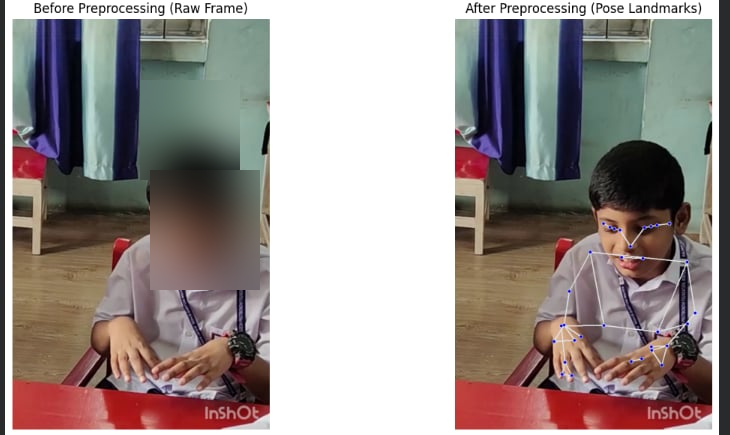
\includegraphics[width=\linewidth]{image/preprocess2.png}
\end{subfigure}
\hfill
\begin{subfigure}{0.32\textwidth}
    \centering
    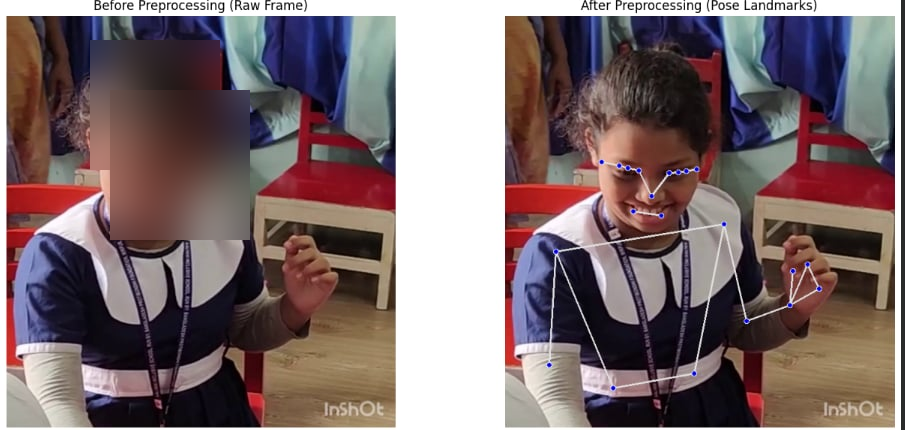
\includegraphics[width=\linewidth]{image/preprocess3.png}
\end{subfigure}

\vspace{0.3cm}

\begin{subfigure}{0.32\textwidth}
    \centering
    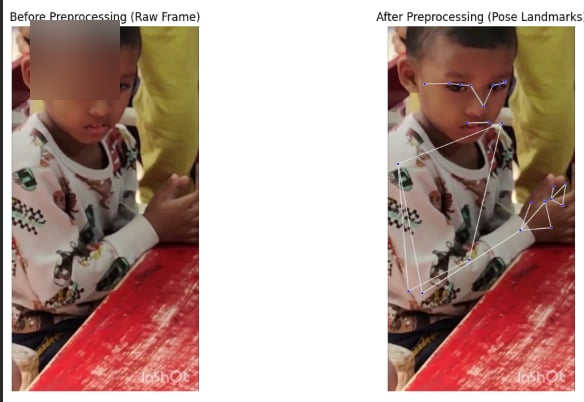
\includegraphics[width=\linewidth]{image/preprocess4.png}
\end{subfigure}
\hfill
\begin{subfigure}{0.32\textwidth}
    \centering
    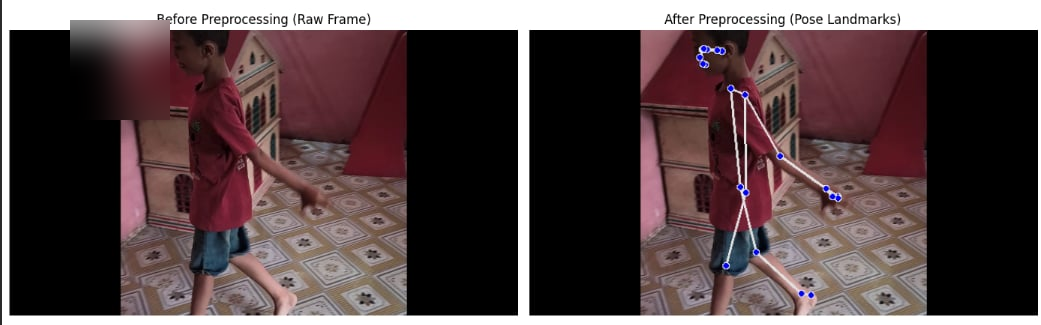
\includegraphics[width=\linewidth]{image/preprocess5.png}
\end{subfigure}
\hfill
\begin{subfigure}{0.32\textwidth}
    \centering
    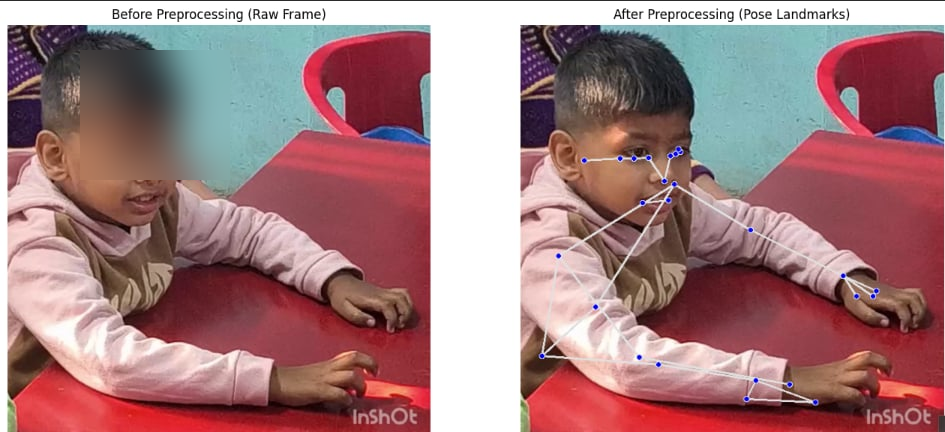
\includegraphics[width=\linewidth]{image/preprocess6.png}
\end{subfigure}

\caption{Before and after preprocessing}
\label{fig:preprocessing_image_before_and_after}
\end{figure*}


As shown in Figure~\ref{fig:preprocessing_image_before_and_after} Each images left sides have been blurred for insuring the chirldrens annonymity, whereas the right side shows the corresponding MediaPipe pose landmark extraction after the preprocessing which is effectively mapping the human body landmarks with pose points and straight lines.

Due to the different length of the videos, sequence normalization is implemented to transform the data into fixed-size of sequences. For the videos with fewer frames then the other ones, the last pose frame is used for padding while for the longer ones, uniform sampling is performed for avoiding overfiting or underfiting issues later in training. 

In addtion and most importantly, data augmentation methods such as temporal cropping, time warping, and flipping are implemented in code to deal with the class imbalance problem.

\begin{table}[]
\centering
\caption{Class Distribution}
\label{tab:class_distribution}
\begin{tabular}{lc}
\toprule
\textbf{Behavior Class} & \textbf{Number of Samples} \\
\midrule
Finger Clipping   & 66\\
Hand Flapping     & 85 \\
Head Touching     & 21 \\
Spinning          & 25 \\
Tilting           & 31 \\
\midrule
\bottomrule
\end{tabular}
\end{table}

As shown in Table~\ref{tab:class_distribution}, our thesis dataset consists of this five behavior and body poses of autism affected child and children did hand flapping more often than anything so this kind of traits are the highest in our dataset. Also, some open source dataset was also included in this thesis to include all races of human. Also there is class imbalance so it was handled using augmentation to get a reliable prediction.




\subsubsection{Feature Extraction and Selection}

For machine learning models which are feature based, statistical features are derived from the pose sequence to evaluate via those models. These features include mean, standard deviation, minimum, maximum, and energy features. The features are derived over the frames in the sequence to make a fixed-dimensional vector for classical classification models.

And also upper-body landmarks have been selected for explanatory analysis, as many autism related behaviors have been greatly expressed by the hand, arm, and head movements specifically.

\subsection{Selected Algorithm Analysis}

For the evaluation of the classification results, various machine learning algorithms are used in this research. Some classical machine learning algorithms used in the study are Random Forest, Support Vector Machine, Logistic Regression, K-Nearest Neighbors, and Gradient Boosting. The extracted statistical features are used for training these models. Ensemble methods are also used for classification with the help of soft voting and hard voting.

In order to directly model the temporal patterns, a Bi-Directional Long Short-Term Memory (BiLSTM) model has been trained on the sequences of poses. This model has been found to be good for modeling short duration repetitive patterns in the videos. Early stopping and class weighting are also employed to avoid overfitting and class imbalance.

Prior studies in the field is valued in our thesis and these alogorithms which are selected are also supported by this prior study. In these studies both classical machine learning and deep leaning approaches have been effectively explored. Such as in the study of \cite{thabtah2018machine} and \cite{duda2016use} they highlighted the effectiveness of traditional machine learning models and in the recent works like of \cite{perochon2023digital} showed the significance of behavioral data driven approaches for early autism detecting while screening.


\subsubsection{Random Forest (RF)}
The Random Forest algorithm is an ensemble-based learning algorithm and it uses multiple decision trees to make up the predictions. The algorithm uses bootstrap sampling and random feature selection to build multiple decision trees and combines their predictions to reduce variance and improve the generalization. In this research, Random Forest is used as baseline algorithm because of its incredible robustness to the noises and its ability to handle non linear decision boundaries in high dimensional feature spaces constructed from pose statistics. Although Random Forest is robust for handling sequential data, it does not actually consider temporal dependencies for short sequences. This choice is supported by early researches where tree based and ensemble learning method have been used and applied in autism classfication tasks where they were able to handle the high dimentional behavioral data \cite{thabtah2018machine,duda2016use}.
\subsubsection{Support Vector Machine (SVM)}
On the other hand, Support Vector Machine is developed for finding the best separating hyperplane that can potentialy maximize the margin of separation. By the help of a kernel function, SVM can effectively handle non linear relationships between the features extracted for the poses. It is also an algorithm which was used in previous researches for generelization of high dimentinal spaces \cite{duda2016use}.
\subsubsection{Logistic Regression (LR)}
Logistic Regression is a Linear Probabilistic Classifier. It uses a logistic function to compute probabilities. Although it is a Linear Classifier, it is still a very good model and can also be used as a baseline model. In this research, it is also used to test whether the least complex models should be used for identifying ASD-related movement patterns. To evalute the need of more complex models, LR has often been used as a baseline in classification problems.\cite{thabtah2018machine}.

\subsubsection{K-Nearest Neighbors (KNN)}
The classifier used is the 'K-Nearest Neighbor' classifier, which is a non-parametric classifier, i.e., it is not dependent on any parameters. It is also called the 'instance-based learner' too, where the classification is done by the voting system of the local neighbors. It is proved to perform good when local patterns are present in the data set. In the present work, the 'KNN classifier' is used to detect the appearing of unique possible local clusters related to ASD behavioral characteristics. For the possiblity of discovering local patterns which can play an important role in classification, KNN has been used as intansce based learning approach \cite{duda2016use}.

\subsubsection{Gradient Boosting (GB)}
Gradient Boosting is a form of Ensemble Learning and it involves a series of weak models such as decision trees that are used to correct errors made by models that are used before it. The optimization process is carried out by minimizing a differentiable function such as the logarithmic function for classification problems using a gradient descent method with respect to different features. GB has ability to reduce classification errors and optimize loss function iteratively thus it can show strong performance in autism related behavioral classification prediction problems \cite{hossain2023smart}.

Gradient Boosting is selected as one of the most important baseline algorithms for our study because of its good bias-variance tradeoff and its ability to achieve a global minimum of the log loss function with validation curves. Unlike the RF algorithm, which reduces the variance of the model by parallel tree generation, the GB algorithm always improves the performance of the model step by step by focusing on samples that are really hard to classify. Thus, it is really useful for small sized datasets used for our study, like the short video-based ASD dataset, and it is a saviour.

In addition, the validation performance of the Gradient Boosting model remains close to the training performance, which shows good generalization and hence less overfitting probability. Thus,this makes it more logical to choose the Gradient Boosting model instead the Random Forest model as the primary classical model.

\subsubsection{Ensemble Voting Methods}
Additionally, in order to enhance the robustness, both soft voting and hard voting ensemble methods are implemented in the code, in which various classical classifiers are combined(high accuracy models). The former is combining of probabilities of classes, whereas in the latter, classes are presented by majority voting. These ensemble methods are useful in overcoming biases of each classifier and making more stable predictions of behavioral classes. To reduce individual model biases and make robust prediction ensemble voting strategy has been also used \cite{rajpurkar2022ai}.\cite{ordonez2016deep} and \cite{zhao2020bidirectional}, these prior works has shown the effectiveness of BiLSTM for sequential data modeling where to recognize human body landmark traits, deep recurrent architectures have shown real effective performance.

\subsubsection{Bi-Directional Long Short-Term Memory (BiLSTM)}
To identify temporal dependency in a more explicit way, a Bi-Directional Long Short-Term Memory network is learned on a fixed-length sequence of poses extracted from the those video clips.And after that this model learns the short-term temporal patterns associated with the repetitive tendency of ASD behaviors. Early stopping is utilized to avoid overfitting cases, while class weighting is used to counterbalance class imbalancings. This BiLSTM model provides a deep learning counterpart to traditional methods and shows a comparison with feature-based learning.

\subsubsection{BiGRU}
The BiGRU model was presented as a lightweight recurrent deep learning architecture designed to capture bidirectional temporal dependencies from the 30-frame pose landmark sequences. BiGRU is more efficient than BiLSTM because it uses fewer gating operations. It also keeps the long-range motion dynamics in autism-related repetitive behaviour clips.Recurrence-based models like GRU are also implemented as working replacements for LSTM in sequence modeling applications and it also ensures comparable results \cite{ordonez2016deep}.

\subsubsection{CNN-BiLSTM}
The CNN-BiLSTM model learns both short-term and long-term patterns of motion by combining one-dimensional convolutional layers with bidirectional LSTM layers. The convolutional layers first take short-term frame-level behavioural features from pose sequences. Then, these features are sent to the BiLSTM layers so that the whole clip can be understood in terms of sequential behaviour.A hybrid approach mixing CNN and LSTM models has proven effective for activity recognition tasks by capturing both spatial and temporal attributes of sequential data \cite{ordonez2016deep}.

\subsection{Explanation of Different Modules}
These components include video preprocessing, pose extraction, sequence normalization, feature extraction, training, evaluation, and prediction. All these components operate independently of each other but as a whole they contribute to the entire process. This is a unique feature of the system that makes it flexible and allows room for further improvement, like adding more behaviors or models.
\subsubsection{Video Preprocessing Module}
The video preprocessing step prepares the raw video clips for the subsequent processing. Since the length of the video clips in our dataset is very small, ranging from 3 to 4 seconds, the video preprocessing step begins by decoding the video frames one by one. It then resizes each frame of the video to a standard size so that all the frames are of the same size. Additionally, it normalizes the frame rate of the video to reduce differences that may arise from different recording by the available equipments.
\subsubsection{Pose Extraction Module}
In this module, we extract the human skeletal features from all frames of the videos using MediaPipe Pose. It is able to locate 33 anatomical keypoints like wrists, elbows, shoulders, hips, knees, and so forth, which are defined by their x, y, and sometimes even z coordinates. It is essentially an informative snapshot of how a person is standing or how they are moving. It is non-intrusive and privacy-friendly compared to RGB data, which is especially useful when working with children or in clinical settings.

\subsubsection{Sequence Normalization Module}
As video clips do not have exactly the same number of frames, we are using a sequence normalization module to normalize all pose sequences to a fixed length of time. All sequences are normalized to 30 frames. Interpolation or uniform sampling have also been performed. It allows the data to be fed to traditional machine learning models that require fixed-length feature vectors, as well as sequence-based deep learning models like BiLSTM.

\subsubsection{Feature Extraction Module}
When it comes to traditional machine learning scenarios, we extract statistical features from the pose sequences, which are normalized. These are features like the average positions, how spread out the coordinates are (standard deviation), as well as how the positions change over time from one frame to the next. These are summarized features, providing us with an efficient representation of the motion, reducing the dimensionality of the data. This makes it more efficient for the traditional classifiers, allowing us to provide interpretability based on what features are most important, as well as other explainable AI techniques for later use.

\subsubsection{Model Training Module}
The training module includes both traditional machine learning algorithms and deep learning models. The traditional models are trained on statistical features extracted from the poses, while the BiLSTM is trained in an end-to-end fashion on the normalized poses. To guarantee the reliability of the performance estimations, we employ hyperparameter tuning and cross-validation. Class weighting is also used to find the imbalance between the ASD behavioral classes during training.
\subsubsection{Evaluation Module}
The evaluation module is to find how well the model performs using general classification performance metrics such as accuracy, precision, recall, F1-score, and confusion matrices. For multiple classes, we use one versus rest ROC curves and their AUC values. To keep the performance metrics stable and unbiased, we use averaging across cross-validation folds.

\subsubsection{Prediction and Deployment Module}
The last module is clearly about prediction of new video clips. When a new video is fed, it goes through the same process of preprocessing, pose extraction, and normalizing data that was performed before, and predictions are made using the models that were previously learned. Such an approach makes it smooth for deployment and opens the way for real-time or assistive use cases  and implementaion opportunity for later for autism behavior analysis.

In this chapter, the proposed approach to the research methodology has been discussed. It has also highlight the proposed framework, data analysis, preprocessing, feature extraction, and the proposed models. A pose-based video analysis system has been proposed to identify autism-related behavioral patterns using traditional machine learning and deep learning techniques. The following chapter is going to discuss the experimental results and evaluate the performance of the proposed system.
